\documentclass[twocolumn,a4j]{jsarticle}
\setlength{\topmargin}{-20.4cm}
\setlength{\oddsidemargin}{-10.4mm}
\setlength{\evensidemargin}{-10.4mm}
\setlength{\textwidth}{18cm}
\setlength{\textheight}{26cm}

\usepackage[top=15truemm,bottom=25truemm,left=15truemm,right=15truemm]{geometry}
\usepackage[latin1]{inputenc}
\usepackage{amsmath}
\usepackage{amsfonts}
\usepackage{amssymb}
\usepackage[dvipdfmx]{graphicx}
\usepackage[dvipdfmx]{color}
\usepackage{listings}
\usepackage{listings,jvlisting}
\usepackage{geometry}
\usepackage{framed}
\usepackage{color}
\usepackage[dvipdfmx]{hyperref}
\usepackage{ascmac}
\usepackage{enumerate}
\usepackage{tabularx}
\usepackage{cancel}
\usepackage{scalefnt}

\renewcommand{\figurename}{Fig.}
\renewcommand{\tablename}{Table }

\lstset{
basicstyle={\ttfamily},
identifierstyle={\small},
commentstyle={\smallitshape},
keywordstyle={\small\bfseries},
ndkeywordstyle={\small},
stringstyle={\small\ttfamily},
frame={tb},
breaklines=true,
columns=[l]{fullflexible},
xrightmargin=0zw,
xleftmargin=3zw,
numberstyle={\scriptsize},
stepnumber=1,
numbersep=1zw,
lineskip=-0.5ex
}

\makeatletter
\def\@maketitle
{
\begin{center}
{\LARGE \@title \par}
\end{center}
\begin{flushright}
{\large 報告書 NO.09 - 1\quad\@date\quad\@author}
\end{flushright}
\par\vskip 1.5em
}
\makeatother

\setcounter{tocdepth}{3}

\author{来代 勝胤}
\title{令和3年度 1月 第1週 報告書}
\date{2022/1/6}

\begin{document}
\columnseprule=0.1mm

\maketitle
\section*{報告内容}
\begin{enumerate}[1.]
    \item 進捗状況
    \item 実験装置の自動化
    \item 評価実験
    \item 補正処理の理論
    \item 校正方法の提案
\end{enumerate}

\section{進捗状況}
自動ステージを用いた実験装置の自動化を目的として実験装置の製作を行った.
また,実験結果の処理方法を検討し,結果として校正実験を行う際に,
その作用力を正しい方向に加えることができれば,ひずみセンサの取付部の状況に関係なく
電圧を作用力へと変換できることがわかった.

\section{実験装置の自動化}
マイクロステージの操作を人為的に行うと
測定時に意図しない電圧変動が起こることや,
操作回数が非常に多くなることから
実験装置の自動化を図った.\\

\subsection{概要}
使用している実験装置にはロードセルを移動させるための地面に対して並行移動するステージと
作用力を与える角度を変化させるための回転ステージが取り付けられている.
この2つのステージを自動ステージヘと換装することで,
実験の効率化とある程度の結果の保証が期待できる.
本実験装置では以下の駿河精機の製品を使用した.

\begin{itemize}
    \item [$\blacksquare$] \textgt{使用した実験装置}
    \item [$\bullet$] 自動ステージコントローラ (DS102)
    \item [$\bullet$] $x$軸マイクロモジュール (PG413-L05AG-C)
    \item [$\bullet$] 自動回転ステージ (KRW06360C-F)
\end{itemize}


\newpage
\section{評価実験}
2021年12月30日(木), 12月31日(金),2022年1月5日(水)に,
製作した実験装置を用いて作用力測定装置の評価実験を行った.\\

\subsection{実験条件}
今回行った実験条件を以下の表1に示す.

\begin{table}[htbp]
    \begin{center}
        \caption{Experimental conditions}
        \begin{tabular}{|p{30mm}|p{20mm}|p{30}|}
            \hline
            \multicolumn{1}{|c|}{\textgt{項目}} & \multicolumn{1}{|c|}{\textgt{条件数}} & \multicolumn{1}{|c|}{\textgt{備考}}                 \\ \hline
            \multicolumn{1}{|c|}{試験片}        & \multicolumn{1}{|c|}{1}               & \multicolumn{1}{|c|}{\textgt{円筒:実験装置で使用}} \\ \hline
            \multicolumn{1}{|c|}{測定角度}      & \multicolumn{1}{|c|}{24}              & \multicolumn{1}{|c|}{\textgt{15度ごとの測定}}       \\ \hline
            \multicolumn{1}{|c|}{試行回数}      & \multicolumn{1}{|c|}{3}               & \multicolumn{1}{|c|}{\textgt{}}                     \\ \hline
        \end{tabular}
    \end{center}
\end{table}

\subsection{実験方法}
今回の実験では,以前行った模擬実験の方法をもとに検討し,
以下のように設定した.\\

$\blacksquare$ \textgt{測定条件}
\begin{itemize}
    \item サンプリング周期は5[Hz]とする
    \item ロードセルをマイクロステージを用いて\\
          0.03 [mm] ずつ移動させ,
          作用力を加え電圧を測定する
    \item 基準を0[mm]として,0.03[mm],0.06[mm],0.09[mm],0.12[mm]の計4回移動させる
\end{itemize}

$\blacksquare$ \textgt{測定準備}
\begin{enumerate}[(1)]
    \item ロードセルを測定する角度に固定
    \item 粗動用ダイヤルでロードセルを大まかな位置に設定
    \item マイクロステージを動かしてロードセルが供試体に接触する位置を0.01[mm]単位で特定
    \item その位置を基準に測定を開始する
\end{enumerate}

$\blacksquare$ \textgt{測定方法}
\begin{enumerate}[(1)]
    \item 測定開始から60秒間待機する
    \item 測定 (40秒間)
    \item 自動ステージ動作時間 (60秒間)
    \item [※] 動作後,電圧の安定を図るため
    \item (2),(3)の作業を5回繰り返す (100秒周期)
    \item [※] 5回目はロードセル,供試体を非接触状態にする
\end{enumerate}

\subsection{実験結果}

以下のFig.1,Fig.2,Table.2に各角度における出力電圧の傾きについての実験結果を示す.
なお,示している数値は実験結果の平均値である.

\begin{figure}[htbp]
    \footnotesize
    \begin{center}
        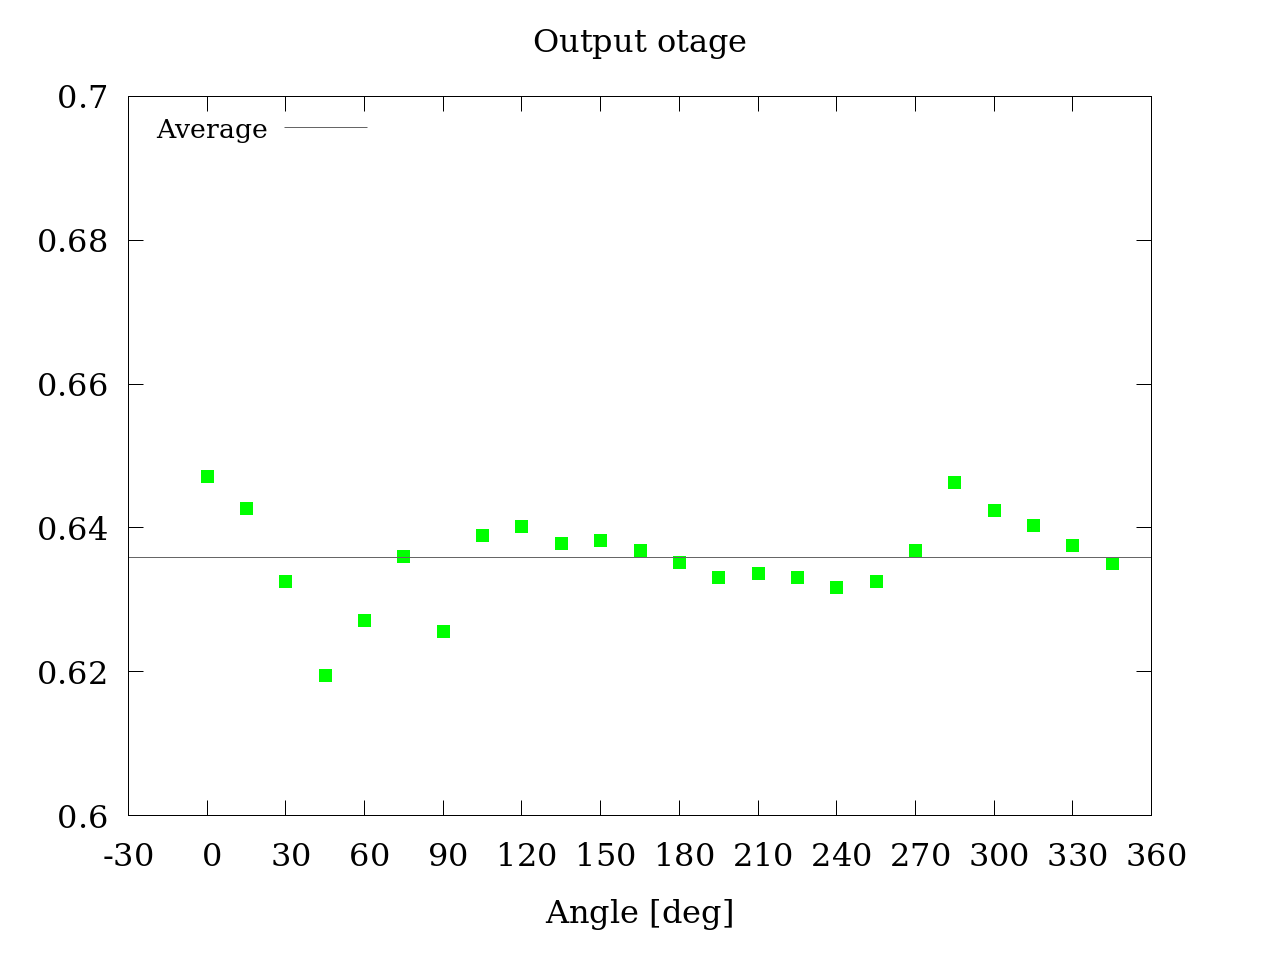
\includegraphics[width=86mm]{../graphes/1-1/05/05_summary-outputvoltage.png}
        \caption{}
        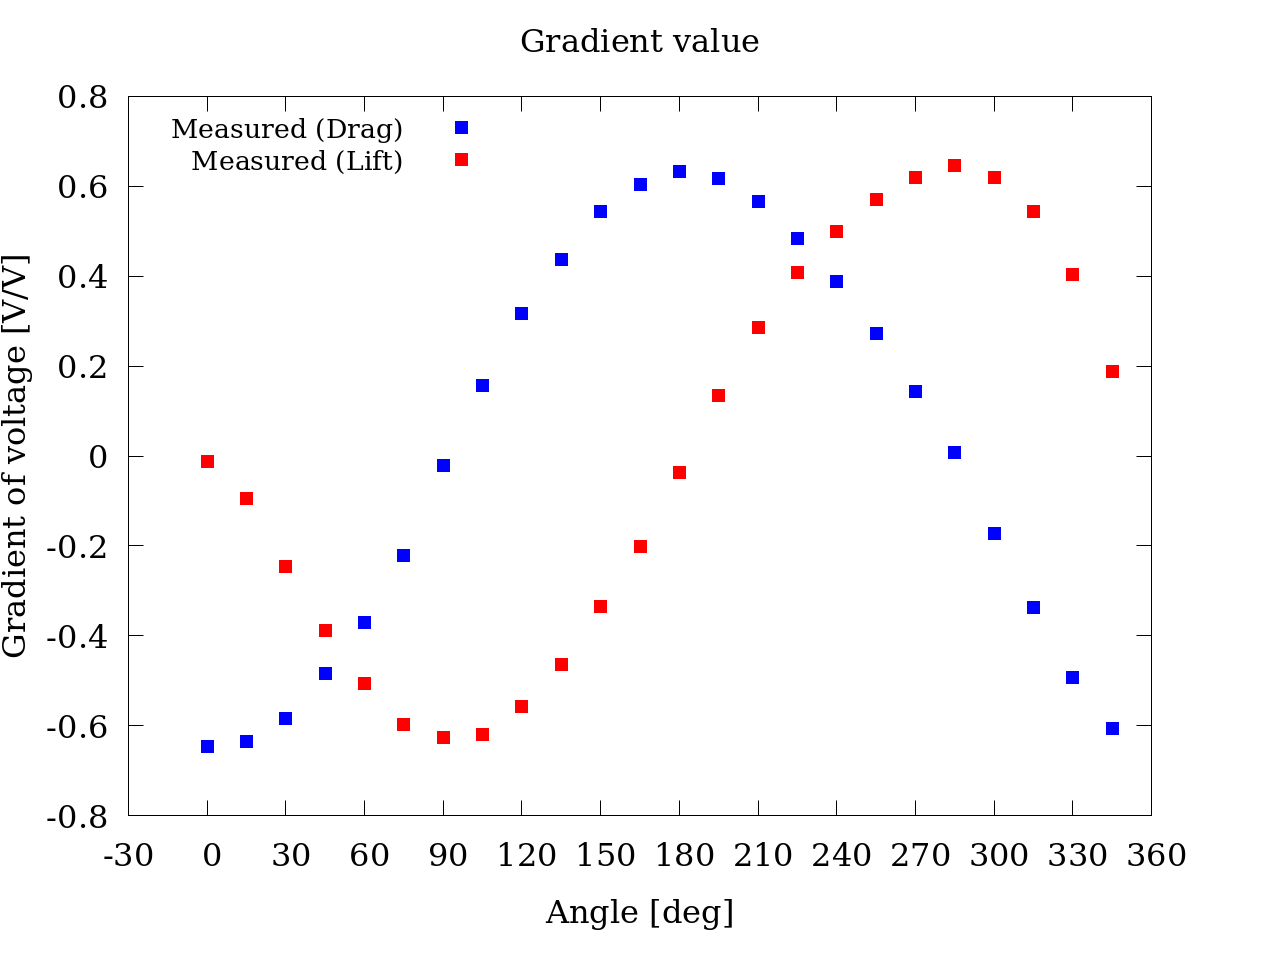
\includegraphics[width=86mm]{../graphes/1-1/05/05_summary-wave.png}
        \caption{}
    \end{center}
\end{figure}

\newpage

\begin{table}[htbp]
    \begin{center}
        \caption{Result summary}
        \begin{tabular}{|p{20mm}|p{20mm}|p{20mm}|}
            \hline
            \multicolumn{1}{|c|}{\textgt{Angle [deg]}} & \multicolumn{1}{|c|}{\textgt{$A_d$ [V/V]}} & \multicolumn{1}{|c|}{\textgt{$A_l$ [V/V]}} \\ \hline
            \multicolumn{1}{|c|}{0}                    & \multicolumn{1}{|r|}{}                     & \multicolumn{1}{|r|}{\textgt{}}            \\ \hline
            \multicolumn{1}{|c|}{15}                   & \multicolumn{1}{|r|}{}                     & \multicolumn{1}{|r|}{\textgt{}}            \\ \hline
            \multicolumn{1}{|c|}{30}                   & \multicolumn{1}{|r|}{}                     & \multicolumn{1}{|r|}{\textgt{}}            \\ \hline
            \multicolumn{1}{|c|}{45}                   & \multicolumn{1}{|r|}{}                     & \multicolumn{1}{|r|}{\textgt{}}            \\ \hline
            \multicolumn{1}{|c|}{60}                   & \multicolumn{1}{|r|}{}                     & \multicolumn{1}{|r|}{\textgt{}}            \\ \hline
            \multicolumn{1}{|c|}{75}                   & \multicolumn{1}{|r|}{}                     & \multicolumn{1}{|r|}{\textgt{}}            \\ \hline
            \multicolumn{1}{|c|}{90}                   & \multicolumn{1}{|r|}{}                     & \multicolumn{1}{|r|}{\textgt{}}            \\ \hline
            \multicolumn{1}{|c|}{105}                  & \multicolumn{1}{|r|}{}                     & \multicolumn{1}{|r|}{\textgt{}}            \\ \hline
            \multicolumn{1}{|c|}{120}                  & \multicolumn{1}{|r|}{}                     & \multicolumn{1}{|r|}{\textgt{}}            \\ \hline
            \multicolumn{1}{|c|}{135}                  & \multicolumn{1}{|r|}{}                     & \multicolumn{1}{|r|}{\textgt{}}            \\ \hline
            \multicolumn{1}{|c|}{150}                  & \multicolumn{1}{|r|}{}                     & \multicolumn{1}{|r|}{\textgt{}}            \\ \hline
            \multicolumn{1}{|c|}{165}                  & \multicolumn{1}{|r|}{}                     & \multicolumn{1}{|r|}{\textgt{}}            \\ \hline
            \multicolumn{1}{|c|}{180}                  & \multicolumn{1}{|r|}{}                     & \multicolumn{1}{|r|}{\textgt{}}            \\ \hline
            \multicolumn{1}{|c|}{195}                  & \multicolumn{1}{|r|}{}                     & \multicolumn{1}{|r|}{\textgt{}}            \\ \hline
            \multicolumn{1}{|c|}{210}                  & \multicolumn{1}{|r|}{}                     & \multicolumn{1}{|r|}{\textgt{}}            \\ \hline
            \multicolumn{1}{|c|}{225}                  & \multicolumn{1}{|r|}{}                     & \multicolumn{1}{|r|}{\textgt{}}            \\ \hline
            \multicolumn{1}{|c|}{240}                  & \multicolumn{1}{|r|}{}                     & \multicolumn{1}{|r|}{\textgt{}}            \\ \hline
            \multicolumn{1}{|c|}{255}                  & \multicolumn{1}{|r|}{}                     & \multicolumn{1}{|r|}{\textgt{}}            \\ \hline
            \multicolumn{1}{|c|}{270}                  & \multicolumn{1}{|r|}{}                     & \multicolumn{1}{|r|}{\textgt{}}            \\ \hline
            \multicolumn{1}{|c|}{286}                  & \multicolumn{1}{|r|}{}                     & \multicolumn{1}{|r|}{\textgt{}}            \\ \hline
            \multicolumn{1}{|c|}{300}                  & \multicolumn{1}{|r|}{}                     & \multicolumn{1}{|r|}{\textgt{}}            \\ \hline
            \multicolumn{1}{|c|}{315}                  & \multicolumn{1}{|r|}{}                     & \multicolumn{1}{|r|}{\textgt{}}            \\ \hline
            \multicolumn{1}{|c|}{330}                  & \multicolumn{1}{|r|}{}                     & \multicolumn{1}{|r|}{\textgt{}}            \\ \hline
            \multicolumn{1}{|c|}{345}                  & \multicolumn{1}{|r|}{}                     & \multicolumn{1}{|r|}{\textgt{}}            \\ \hline \hline
            \multicolumn{1}{|c|}{Average}              & \multicolumn{1}{|r|}{}                     & \multicolumn{1}{|r|}{\textgt{}}            \\ \hline
        \end{tabular}
    \end{center}
\end{table}

\newpage

\section{補正処理の理論}
実験を行う過程で,作用力測定装置と回流水槽等の作用力を与える装置を
正しく設置することが非常に困難であることがわかった.
そこで,事前に作用力測定装置のひずみセンサー取付部について,
角度に対する出力電圧の特性を調べ,その結果を用いて,
後に行う校正実験結果に有効的な補正処理方法を検討した.\\

\subsection{校正時の問題点}
校正実験を行い,出力電圧を評価するためには
それぞれの実験装置を正しい方向(角度)に設置する必要がある.
しかし,これまでの実験過程及び結果から,
以下のような要因が校正実験の際に影響を与えていることがわかった.

\begin{itemize}
    \item [$\bullet$] 抗力・揚力方向のひずみセンサが直角に取り付けられていない
    \item [$\bullet$] ひずみセンサ取付部が測定装置の正しく取り付けられていない
    \item [$\bullet$] 実験装置が水流に対して正しい方向に設置されていない
    \item [$\bullet$] 校正装置が正しく取り付けられていない
\end{itemize}

\subsection{座標軸の回転による影響}
ここで,作用力の座標軸について抗力方向を$x軸$,揚力方向を$y$軸,
同様にひずみセンサの座標軸について抗力・揚力方向をそれぞれ$x'$軸,$y'$軸とすると
上記の校正時の問題点により,以下の図のように
ひずみセンサの$x'$軸,$y'$軸は,$x$軸,$y$軸に対して
それぞれ角度$\theta_1$,$\theta_2$だけ
ズレが生じていると考えられる.\\

\begin{figure}[htbp]
    \footnotesize
    \begin{center}
        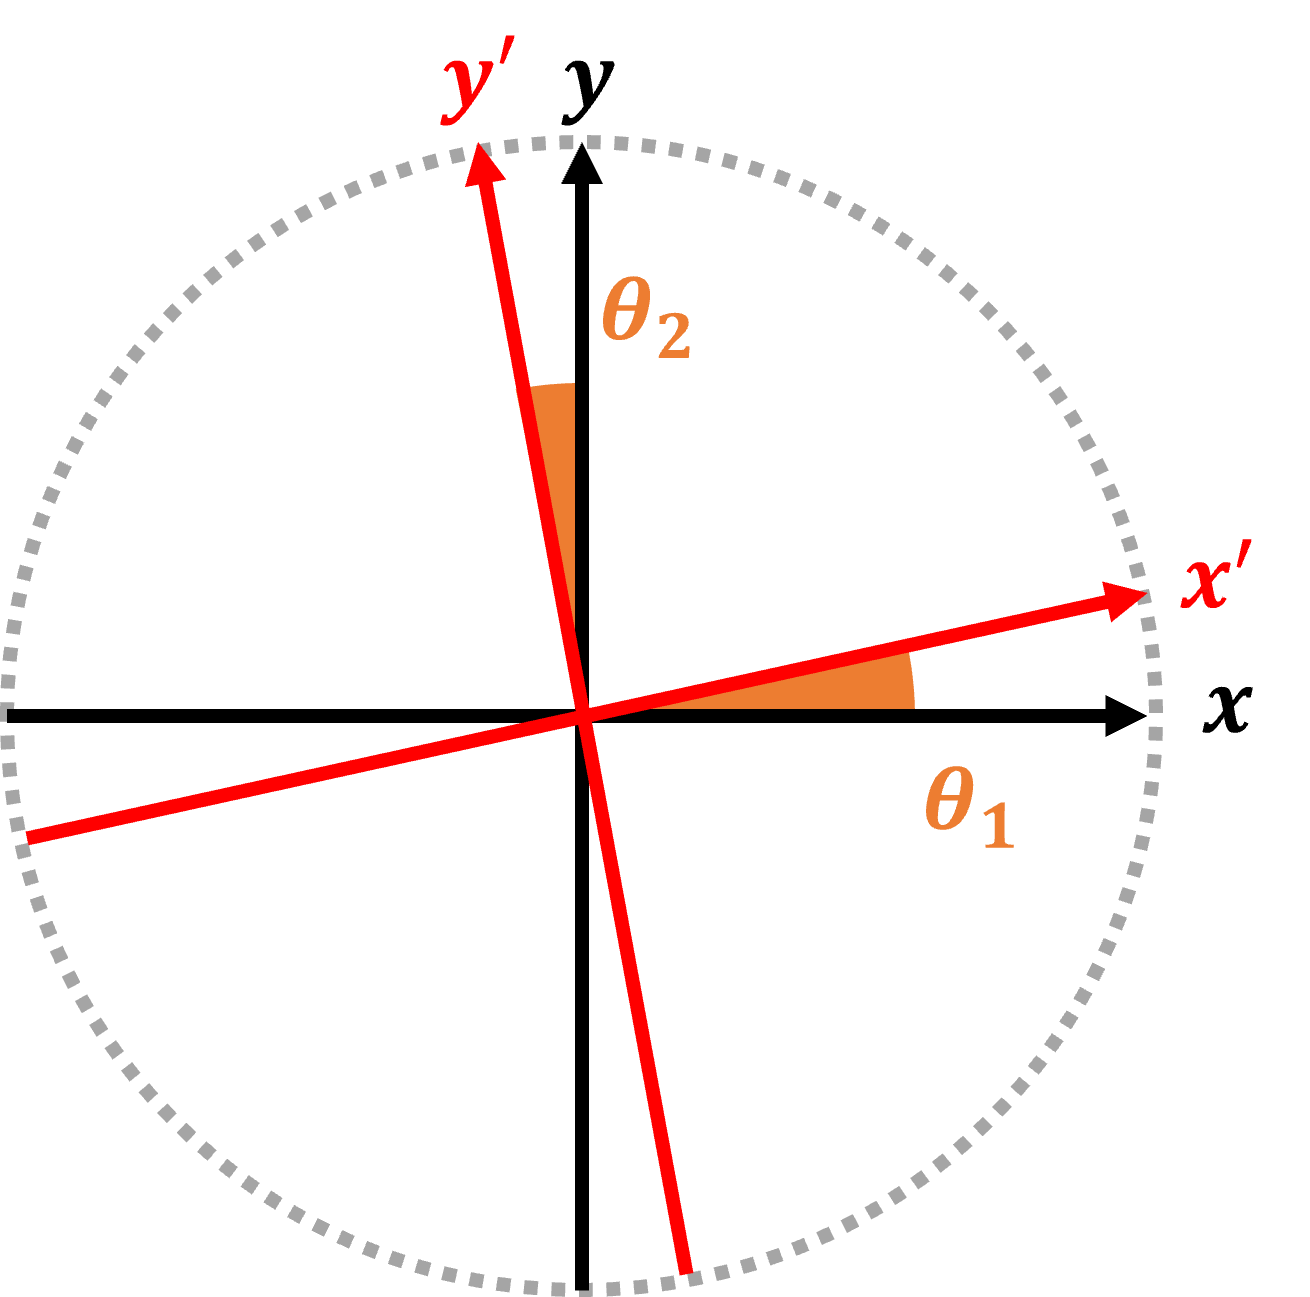
\includegraphics[width=60mm]{../images/image_1.png}
        \caption{}
    \end{center}
\end{figure}

\newpage

このとき,作用力$F$が加えられたとき,
それぞれの方向に以下の図のような作用力$F_x$,$F_y$, $F_{x'}$,$F_{y'}$が加わる.

\begin{figure}[htbp]
    \footnotesize
    \begin{center}
        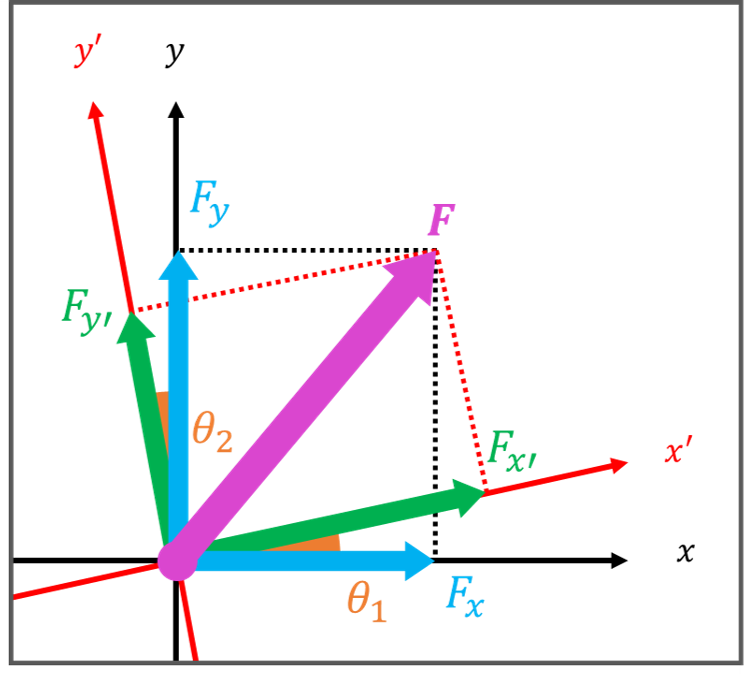
\includegraphics[width=70mm]{../images/image_2.png}
        \caption{}
    \end{center}
\end{figure}

ここで,測定装置から得られる出力電圧は$F_{x'}$および,$F_{y'}$に起因するものであり,
作用力を評価するためには,この電圧を本来の抗力・揚力方向である$x$軸,$y$軸方向(以後,正規座標系とする)の電圧に変換し,
作用力へと換算する必要がある.\\

\subsection{位相角の算出}
まずはじめに,座標軸においてそれぞれの角度のズレ$\theta_1$,$\theta_2$の大きさを調べる必要がある.
評価実験結果から算出された,各角度に対する出力電圧の傾きの大きさの値から
正弦波状の結果を得ることができた.
ここで,離散フーリエ変換を適用し,波数1の成分について位相角を算出することで
理論上の位相との位相差を求めることができる.

\begin{itemize}
    \item [$\blacksquare$] 位相角$\phi$の算出
          \begin{eqnarray*}
              \mathrm{\phi \; [deg]} = \arctan \left(\frac{Im}{Re}\right) × \frac{180}{\pi}
          \end{eqnarray*}
    \item [※] 位相角$\phi$は,フーリエ変換の性質上,余弦波に対する位相角を示している.
\end{itemize}

また,各角度に対する出力電圧の傾きの大きさについて,
抗力・揚力方向の理論式は抗力方向の出力電圧を$V_{x}$,揚力方向の出力電圧を$V_{y}$として以下のように表される.

\begin{itemize}
    \item [$\blacksquare$] \textgt{抗力・揚力における出力電圧の理論式}
          \begin{eqnarray*}
              V_{x} &=& A \sin\left(\omega t + \frac{3}{2}\pi\right) = A \cos\left(\omega t + \pi\right)\\
              V_{y} &=& A \sin\left(\omega t + \pi\right) = A \cos\left(\omega t + \frac{1}{2}\pi\right)
          \end{eqnarray*}
    \item [※] $A$ は定数
\end{itemize}

したがって,算出した位相角を抗力・揚力方向についてそれぞれ$\phi_1$,$\phi_2$とすると,
理論値との位相差$\theta_1$,$\theta_2$は以下のように算出される.

\begin{itemize}
    \item [$\blacksquare$] \textgt{抗力・揚力における出力電圧の位相差の算出}
          \begin{eqnarray*}
              \theta_1 &=& \pi - \phi_1\\
              \theta_2 &=& \frac{1}{2} \pi - \phi_2
          \end{eqnarray*}
\end{itemize}

これより,Fig.1における波形はそれぞれの方向について$\theta_1$,$\theta_2$だけ
遅れているということがわかる.
すなわち,Fig.について,座標軸$x'$軸,$y'$軸は左回りを正の方向として,
正規座標系に対してそれぞれ$\theta_1$,$\theta_2$だけ回転していることになる.\par

また,抗力・揚力方向ひずみセンサの取付角$\phi$は,
ひずみセンサにおける抗力・揚力方向の位相角$\phi_1$,$\phi_2$の差から
求めることができる.

\begin{itemize}
    \item [$\blacksquare$] 抗力・揚力方向のひずみセンサの取付角度 $\phi$
          \begin{eqnarray*}
              \phi &=& \left| \phi_x - \phi_y \right| \\
          \end{eqnarray*}
\end{itemize}

\subsection{出力電圧の座標変換}
位相角$\theta_1$,$\theta_2$が求められたことから,それらを用いて座標変換を行う.
ここで,ひずみゲージにおける抗力・揚力方向座標軸である$x'$軸,$y'$軸を
それぞれ$f_{x1}\left(x\right)$,$f_{y1}\left(x\right)$として,
正規座標軸の$x$を用いた式で表す.

\begin{figure}[htbp]
    \footnotesize
    \begin{center}
        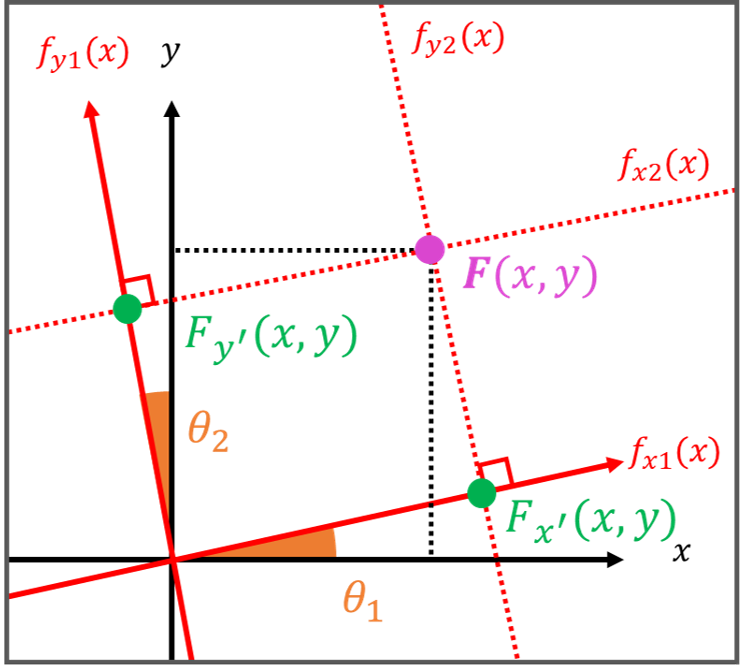
\includegraphics[width=70mm]{../images/image_3.png}
        \caption{}
    \end{center}
\end{figure}

算出した位相角$\theta_1$,$\theta_2$より,$f_{x1}\left(x\right)$,$f_{y1}\left(x\right)$は
以下のように表される.

\begin{itemize}
    \item [$\blacksquare$] $f_{x1}\left(x\right)$,$f_{y1}\left(x\right)$の算出
          \begin{eqnarray*}
              f_{x1}\left(x\right) &=& \tan \theta_1 \; x\\
              f_{y1}\left(x\right) &=& - \frac{1}{\tan \theta_2}\; x
          \end{eqnarray*}
\end{itemize}

このとき,作用力$F$は,Fig.に示す点$F$の座標を表すベクトルと考えることができる.
また,その座標はFig.より,$f_{x1}\left(x\right)$,$f_{y1}\left(x\right)$の法線で,
点$F_{x'}$,$F_{y'}$を通る直線,
$f_{x2}\left(x\right)$,$f_{y2}\left(x\right)$の交点であることがわかる.\par
ここで,ひずみゲージから得ることのできる出力電圧の傾きから,
$F_{x'}$,$F_{y'}$のベクトルの大きさ$|\boldsymbol{F_{x'}}|$,$|\boldsymbol{F_{y'}}|$を
得ることができる.
角度$\theta_1$,$\theta_2$が求められていることから,
点$F_x'$,$F_y'$の座標は以下のように求めることができる.

\begin{itemize}
    \item [$\blacksquare$] 点$F_x'$,$F_y'$の座標
          \begin{eqnarray*}
              F_{x'} \left(x ,y\right) &=& \left(|\boldsymbol{F_{x'}}| \cos \theta_1,\; |\boldsymbol{F_{x'}}| \sin \theta_2\right)\\
              F_{y'} \left(x ,y\right) &=& \left( - |\boldsymbol{F_{y'}}| \sin \theta_1,\; |\boldsymbol{F_{y'}}| \cos \theta_2\right)
          \end{eqnarray*}
\end{itemize}

次に,直線$f_{x2}\left(x\right)$,$f_{y2}\left(x\right)$を求める.
$f_{x1}\left(x\right)$,$f_{y1}\left(x\right)$,点$F_x'$,$F_y'$の座標の座標から
それぞれ以下のように算出される.

\begin{itemize}
    \item [$\blacksquare$] $f_{x2}\left(x\right)$,$f_{y2}\left(x\right)$の算出
          \begin{eqnarray*}
              f_{x2}\left(x\right) &=& - \frac{1}{\tan \theta_1} \; x + \frac{|F_{x'}|}{\sin \theta_1}\\
              f_{y2}\left(x\right) &=& \tan \theta_2\; x + \frac{|F_{y'}|}{\cos \theta_2}
          \end{eqnarray*}
\end{itemize}

以上の$f_{x2}\left(x\right)$,$f_{y2}\left(x\right)$から,
交点の座標$F\left(x,y\right)$を求めると以下のようになる.

\begin{itemize}
    \item [$\blacksquare$] $F\left(x,y\right)$の算出
          \begin{eqnarray*}
              x
          \end{eqnarray*}
\end{itemize}

したがって,正規座標系における抗力$F_x$および揚力$F_y$は,以下のように表される.

\begin{itemize}
    \item [$\blacksquare$] 抗力$F_x$・揚力$F_y$の大きさ
          \begin{eqnarray*}
              F_x &=& \\
              F_y &=&
          \end{eqnarray*}
\end{itemize}

以上の過程よりひずみセンサにおける座標系から正規座標系への変換が可能である.

\newpage

\subsection{テストデータへの適用}
抗力$F_x$・揚力$F_y$を導出する補正理論について
テストデータを作成し,それに適用することでその有効性を確かめた.

\begin{itemize}
    \item [$\blacksquare$] \textgt{$\theta_1 = 15 \; \mathrm{[deg]}$,$\theta_2 = 20 \; \mathrm{[deg]}$のとき}\\
          \begin{figure}[htbp]
              \footnotesize
              \begin{center}
                  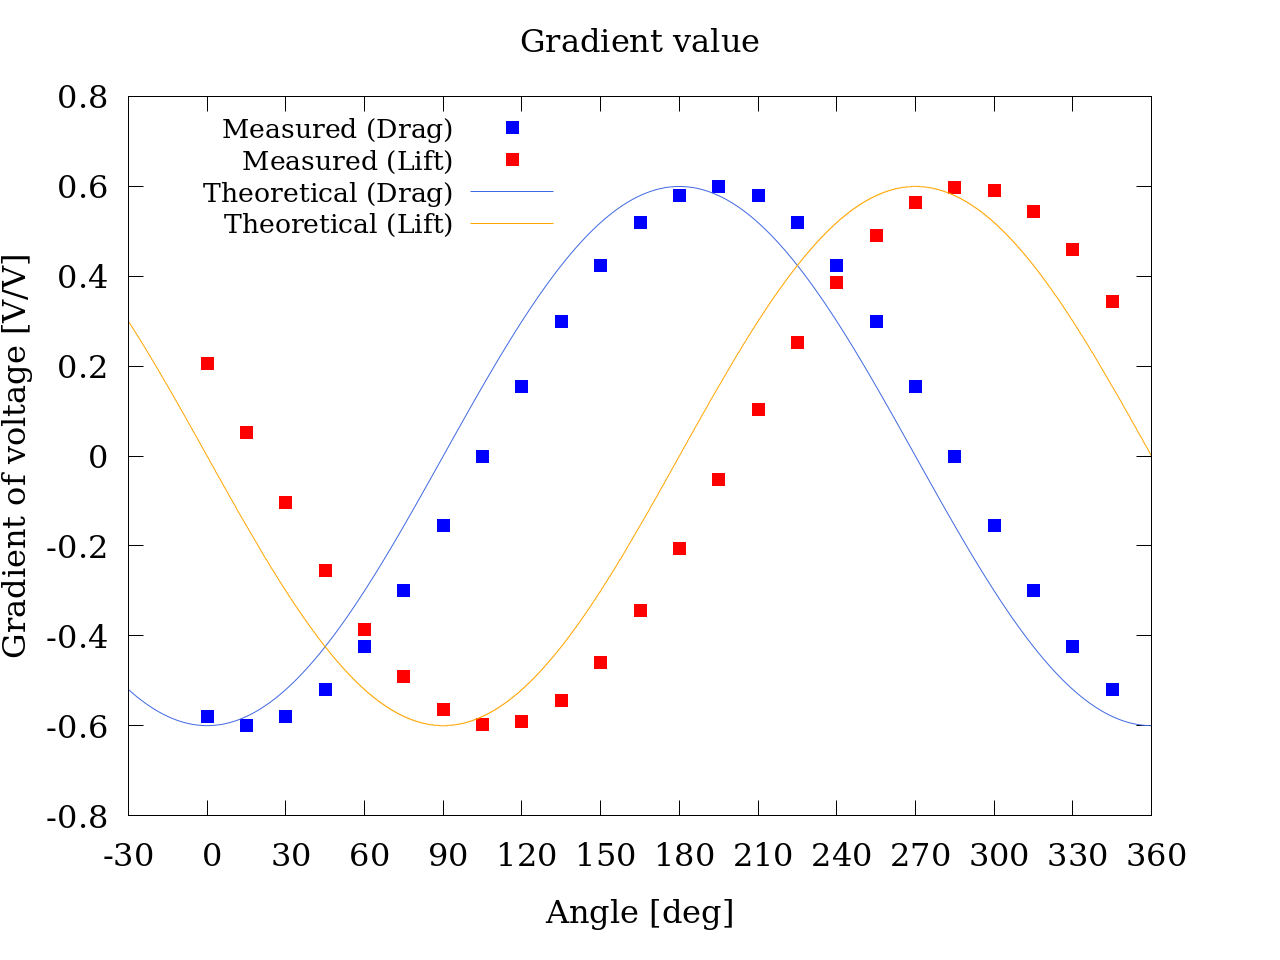
\includegraphics[width=86mm]{../graphes/simulation_150_200/20/20_adjust-value.png}
                  \caption{}
                  \includegraphics[width=86mm]{../graphes/simulation_150_200/21/21-2_corrected_drag.png}
                  \caption{}
                  \includegraphics[width=86mm]{../graphes/simulation_150_200/21/21-2_corrected_lift.png}
                  \caption{}
              \end{center}
          \end{figure}
          \newpage
    \item [$\blacksquare$] \textgt{$\theta_1 = -15 \; \mathrm{[deg]}$,$\theta_2 = -20 \; \mathrm{[deg]}$のとき}\\
          \begin{figure}[htbp]
              \footnotesize
              \begin{center}
                  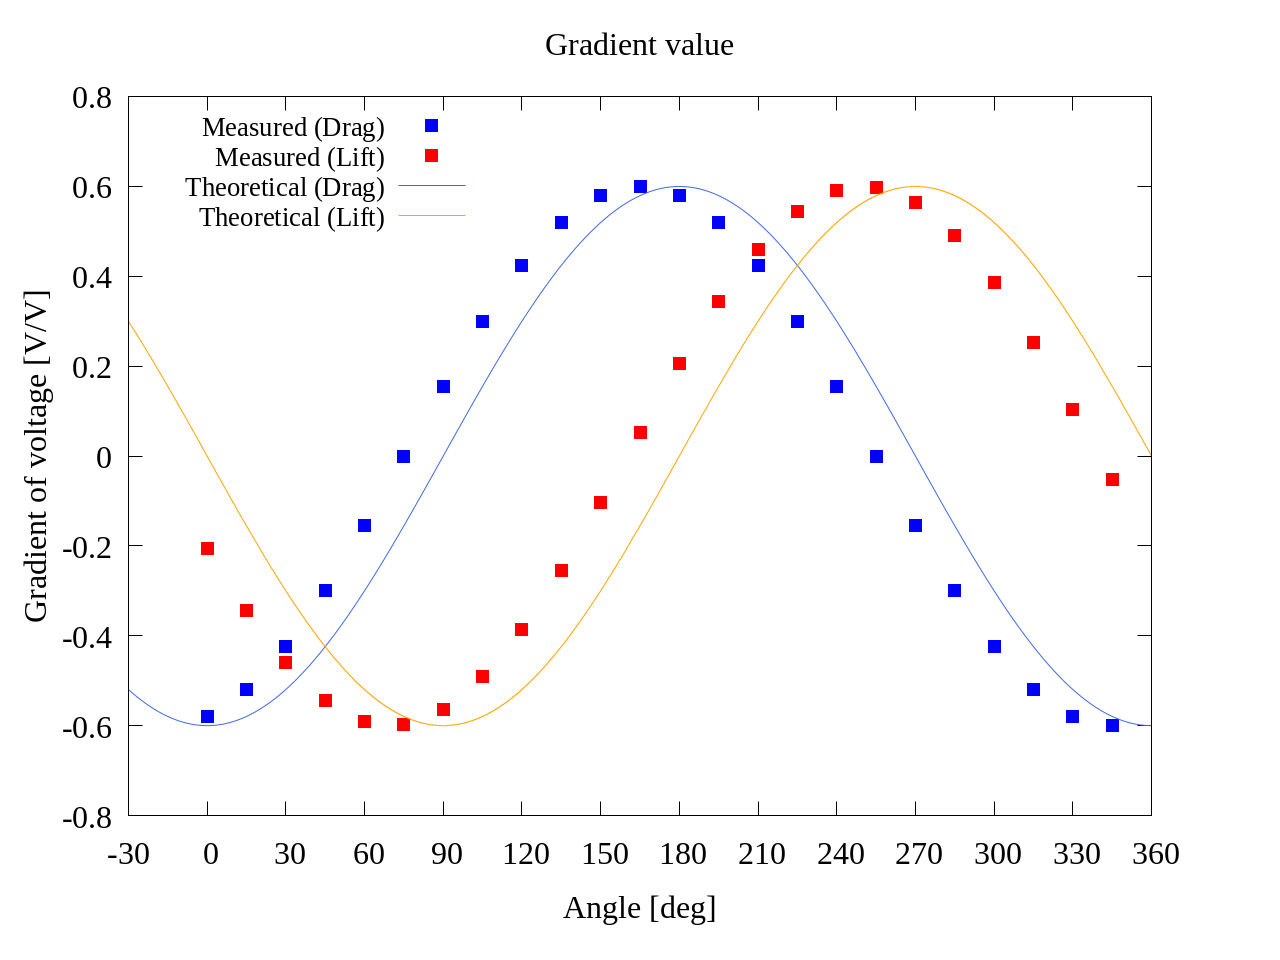
\includegraphics[width=86mm]{../graphes/simulation_-150_-200/20/20_adjust-value.png}
                  \caption{}
                  \includegraphics[width=86mm]{../graphes/simulation_-150_-200/21/21-2_corrected_drag.png}
                  \caption{}
                  \includegraphics[width=86mm]{../graphes/simulation_-150_-200/21/21-2_corrected_lift.png}
                  \caption{}
              \end{center}
          \end{figure}
          \newpage
    \item [$\blacksquare$] \textgt{$\theta_1 = 90 \; \mathrm{[deg]}$,$\theta_2 = 90 \; \mathrm{[deg]}$のとき}\\
          \begin{figure}[htbp]
              \footnotesize
              \begin{center}
                  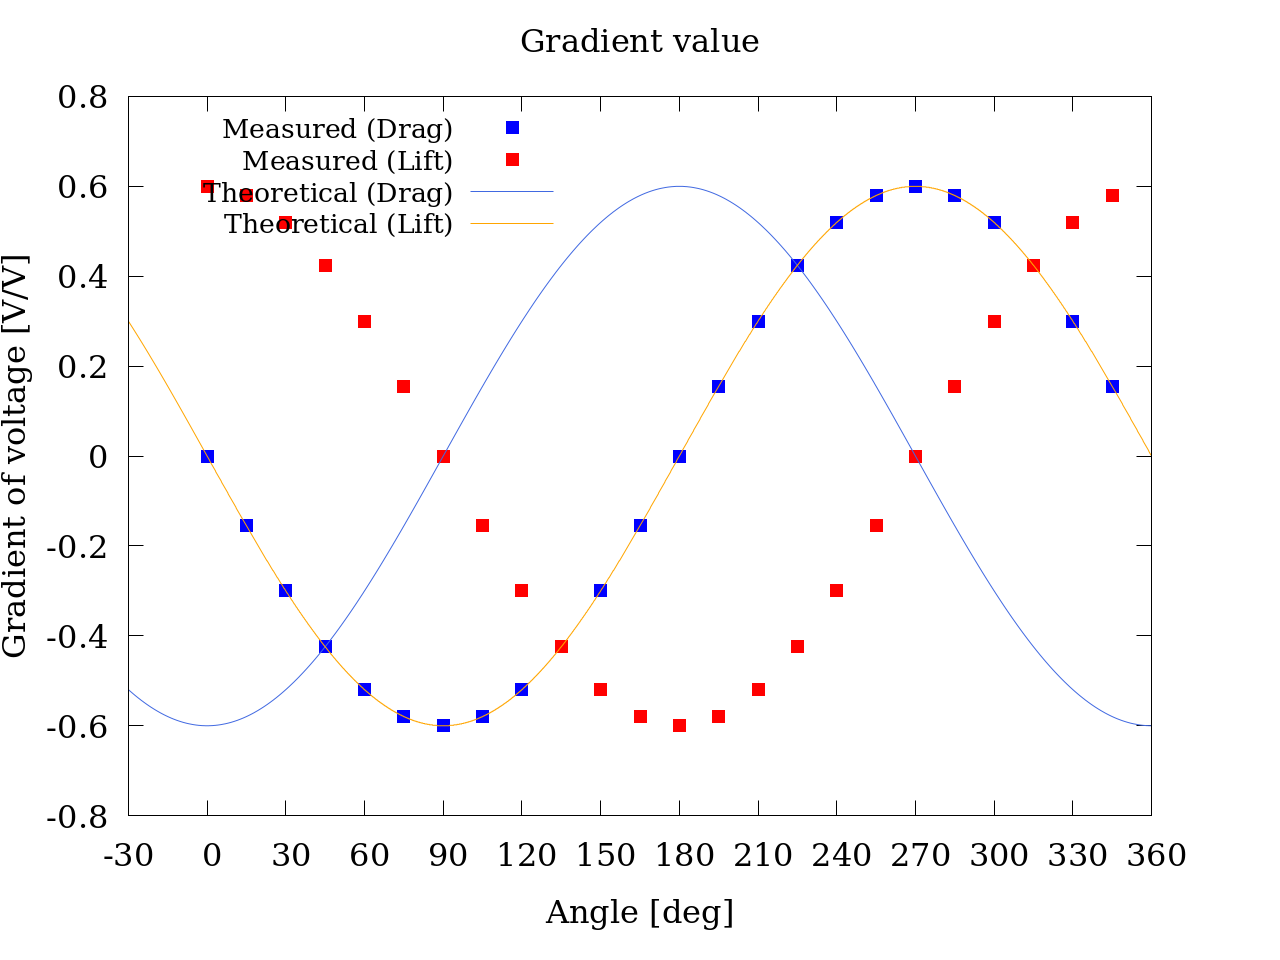
\includegraphics[width=86mm]{../graphes/simulation_900_900/20/20_adjust-value.png}
                  \caption{}
                  \includegraphics[width=86mm]{../graphes/simulation_900_900/21/21-2_corrected_drag.png}
                  \caption{}
                  \includegraphics[width=86mm]{../graphes/simulation_900_900/21/21-2_corrected_lift.png}
                  \caption{}
              \end{center}
          \end{figure}
    \item [※] 振幅は,実験結果を基準に0.6と設定している.
          \newpage
\end{itemize}

\section{校正方法の提案}
\end{document}